\section{Exploring Structure through Scattering}\label{ch1:sec1:background}

    %\subsection{Discovery of the Nucleons}
    The typical length scales for atoms and nucleons are 0.1 nm which is far smaller than the wavelength of human-visible light ($\sim$ 500 nm). As such, atomic and nuclear structure must be explored by forcing some interaction and then inferring the structure from the observed results. Thomson's atomic model was famously tested in the early 1900s by Ernest Rutherford's research group, wherein $\alpha$ particles were fired at thin metal targets, and the scattering behaviour was observed \cite{Geiger1909OnAlpha-Particles} \cite{Rutherford1911TheAtom}. 
    
    The results were not consistent with Thomson's model, but instead indicated that there was a very small, dense, positively charged nucleus at the center of every atom. Further experiments by Rutherford would lead to the discovery of the proton around 1920 \cite{Rutherford1919CollisionNitrogen}. Puzzles about the nucleus remained, including a consistent description of isotopes, until 12 years later when James Chadwick suggested the existence of the neutron \cite{Chadwick1932PossibleNeutron}. With electrons and the two nucleons discovered, it seemed as though the indivisible constituents of the atom were finally realized, but future experiments showed a much more complex, sub-nuclear structure. 
    
    \subsection{Scattering at Different Resolution Scales}

        The diffraction limit for microscopic (compared to telescopic) systems can be approximated by equation \ref{eq:diffraction}, where \textit{n} is the index of refraction, $\theta$ is a measure of the device aperture, $\lambda$ is the wavelength of the probe, and \textit{d} is the minimum resolvable length scale. Thus, the wavelength of a probe sets a fundamental lower limit on the achievable resolution of a microscopic imaging system - roughly, at small enough distances, the probe's waves interfer, prohibiting resolution at or below that scale. 
    
        \begin{equation}\label{eq:diffraction}
            d = \frac{\lambda}{2n\sin{\theta}}
        \end{equation}\myequations{Diffraction Limit}
        
        For visible light microscope systems, $\lambda$ $\sim$ 500 nm, and so the minimum resolvable feature size is approximately \textit{d} $\sim$ 250 nm. Techniques exist to extend the resolution size by approximately an order of magnitude, e.g. expansion microscopy \cite{Chen2015ExpansionMicroscopy} or Near-Field Scanning Optical Microscopy \cite{Ma20216nmSource}, but non-visible-light probes are needed for scales below $\sim$ 10 nm. 

        
        %good guide: https://www.thermofisher.com/us/en/home/global/forms/industrial/backscattered-electrons-sem.html
        %Why no proton microscopes? https://physics.stackexchange.com/questions/574802/why-no-proton-microscopes-proton-diffraction-or-proton-scattering-experiments#:~:text=Proton%20crystallography%20is%20not%20typically,neutrons%20with%20the%20same%20energy.
        % Comprehensive book on electron microscopes: https://link.springer.com/book/10.1007/978-0-387-76501-3
        % Details on how to get beyond the diffraction limit with special tricks https://advanced-microscopy.utah.edu/education/super-res/

        In particular, the de Broglie relationship \ref{eq:deBroglie} \cite{Broglie1924XXXV.Quanta/i} states that the wavelength $\lambda$ of a particle is inversely proportional to its momentum \textit{p}, with \textit{h} being Planck's constant. 
        
            \begin{equation}\label{eq:deBroglie}
               \lambda = \frac{h}{p}
            \end{equation}\myequations{de Broglie Relationship}

        With this relationship, we can see that by increasing a particle's momentum, its effective wavelength is reduced. This is the fundamental principle which allows electron microscopes to image matter at a resolution of $\sim$ 10-0.1 nm \cite{Franken2020ADevelopments}, corresponding to electron momentums of $\sim$ 1-100 keV. At this scale, viruses, cells, molecular structures, and even atoms can be imaged \cite{Williams2009TransmissionMicroscopy}, with striking results commonly published online. Other probes could be used circumvent the diffraction limit, such as high energy (low-wavelength) photons or high momentum (low de Broglie wavelength) protons or neutrons, but electrons are an ideal candidate in this regime as they are easy to produce, steer, interact with, and detect. 

        To move beyond imaging at the atomic scale ($\sim$ 1 \AA) to the nuclear scale ($\sim$ 1 fm) requires probes that are 100,000 times more powerful. Electrons are still an ideal probe due to their (apparent) lack of internal structure, but rather than a room sized microscope, an entire accelerator facility is needed to achieve high enough energies and luminosities for sub-nuclear scale resolution. 
        


    \subsection{Elastic Scattering and Form Factors}

        Imaging with electrons (or other non-visible-light probes) at any energy scale is commonly understood in terms of scattering cross sections, $\sigma$, with dimensions of area and interpreted as the probability for a certain interaction to occur. Typical elastic scattering cross sections for transitions metals with 100 keV incident electrons as in electron microscopy are $\sim 10^{-22} m^2$ \cite{Williams2009TransmissionMicroscopy}. In contrast, the cross sections to be discussed in this thesis are on the order of tens of nanobarn ( $10^{-36} m^2$), or 14 orders of magnitude smaller. 
        
       % \begin{figure}[h]
       %     \centering
      %      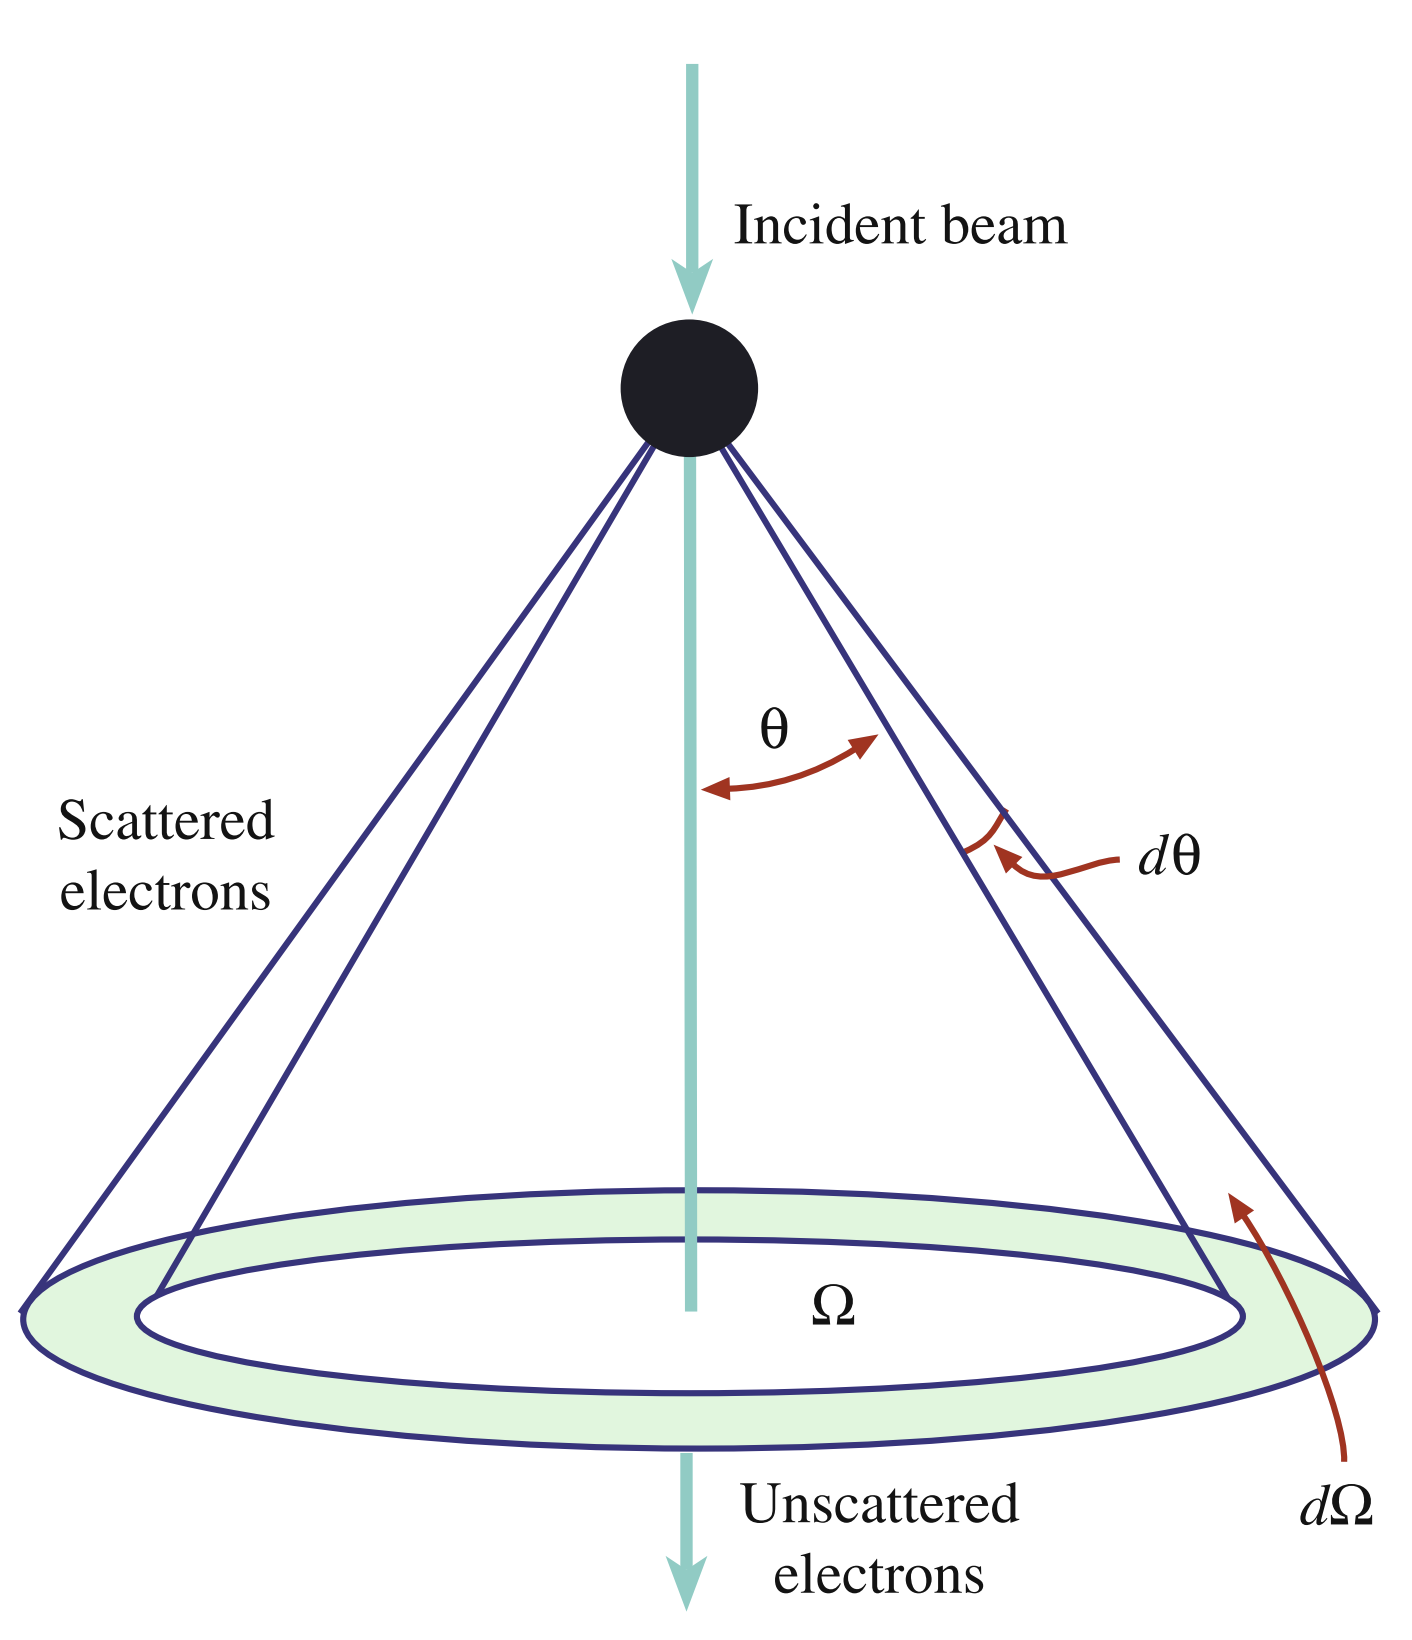
\includegraphics[width=0.5\textwidth]{Chapters/Ch1-Intro/Ch1-Sec1-Background/pics/intro/scattering_geometry.png}
       %     \caption{Geometric relationship between differential scattering angle d$\theta$ and differential solid angle d$\Omega$, from \cite{Williams2009TransmissionMicroscopy} }
      %      \label{fig:GeometricScattering}
      %  \end{figure}

        \begin{figure}[H]
            \centering
            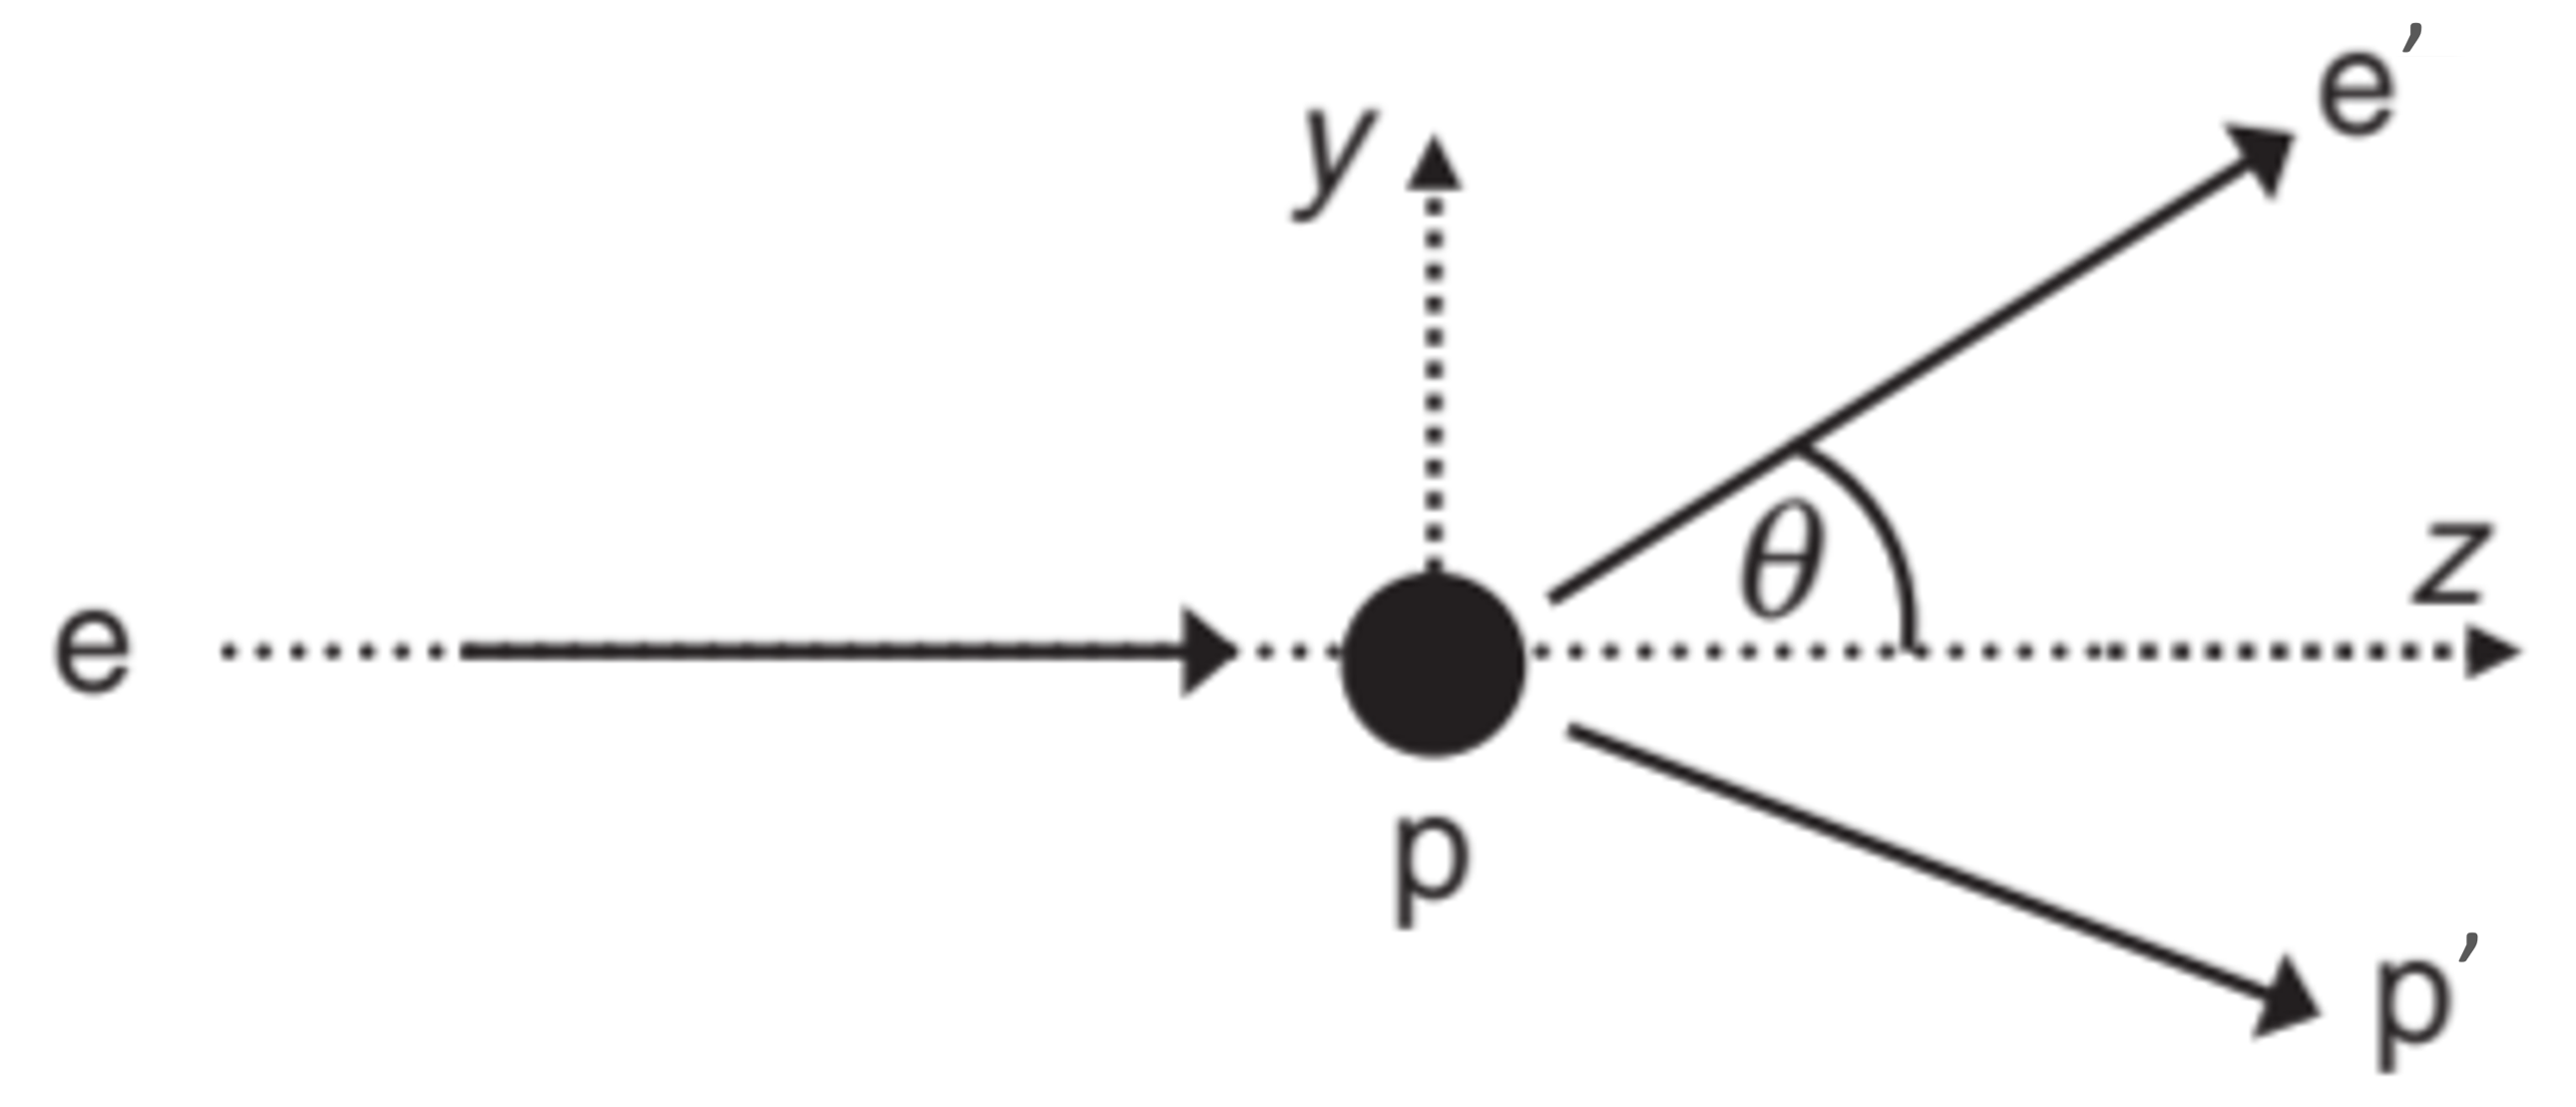
\includegraphics[width=10cm]{Chapters/Ch1-Intro/Ch1-Sec1-Background/pics/elastic-ep/kine-e-2.PNG}
            \caption{Elastic scattering diagram}
        \end{figure}
            
      %  In general, as illustrated in Fig. \ref{fig:GeometricScattering} electrons will scatter through an angle $\theta$ into a solid angle $\Omega$.
        
        
        %as $\Omega = 2\pi(1-\cos{\theta})$, which results in a differential form of $\frac{d\Omega}{d\theta} = 2\pi \sin{\theta}$.

        %From this, we can write the differential cross section as:
        
        %\begin{equation}\label{eq:GeneralDifferentialCrossSection}
        %%   \frac{d\sigma}{d\Omega} = \frac{d\sigma}{d\Omega}\frac{d\Omega}{d\theta} = \frac{1}{2\pi \sin{\theta}}\frac{d\sigma}{d\theta}
        %\end{equation}\myequations{General Differential Cross Section}


        The scattering cross section for a probe (such as an electron) incident on a target, can be calculated at lowest order by considering a fixed (no recoil), point-like (no structure),  radially symmetric Coulomb potential (e.g., a proton) with a non-relativistic incident charged particle. The resulting equation was used by Rutherford's group in the discovery of the nucleus, and for an electron beam of energy  $E_{beam}$ is given by Eq. \ref{eq:RutherfordDiffX}, where $\alpha$ is the fine structure constant.

            \begin{equation}\label{eq:RutherfordDiffX}
                {\frac{\theta}{2}}(\frac{d\sigma}{d\Omega})_{Ruth} = \frac{\alpha^2}{16E^2_{beam}\sin^4{(\theta/2)}}
            \end{equation}
                \myequations{Rutherford Scattering Differential Cross Section}

        To probe smaller resolution scales, it is necessary to increase the energy of the beam, and eventually the probe must be treated relativistically. This correction term is provided by the Mott scattering cross section, given by Eq. \ref{eq:MottDiffX}, which still assumes a fixed, point-like target, with only Coulomb interactions.
            
                \begin{equation}\label{eq:MottDiffX}
                     (\frac{d\sigma}{d\Omega})_{Mott} = \frac{\alpha^2}{4E^2\sin^4{(\theta/2)}}\cos^2{\frac{\theta}{2}} = \left( \frac{\alpha}{2E\sin^2{(\theta/2)}}\cos{\frac{\theta}{2}} \right)^2 = 4\cos^2{\frac{\theta}{2}}(\frac{d\sigma}{d\Omega})_{Ruth}
                \end{equation}
                \myequations{Mott Scattering Differential Cross Section}
        
    
 
         At higher incident electron energies (and thus finer spatial resolutions), the proton's finite size must be accounted for, as well as the momentum transferred to it. The tree-level Feynman diagram for elastic electron-proton scattering is show in in Fig. \ref{fig:feynmanElastic}. The incoming electron \textit{e} exchanges a virtual photon with the proton \textit{p}, resulting in a momentum transfer of $q = p_{e'} - p_{e}$. 
         
        \begin{figure}[H]\label{fig:feynmanElastic}
            \centering
            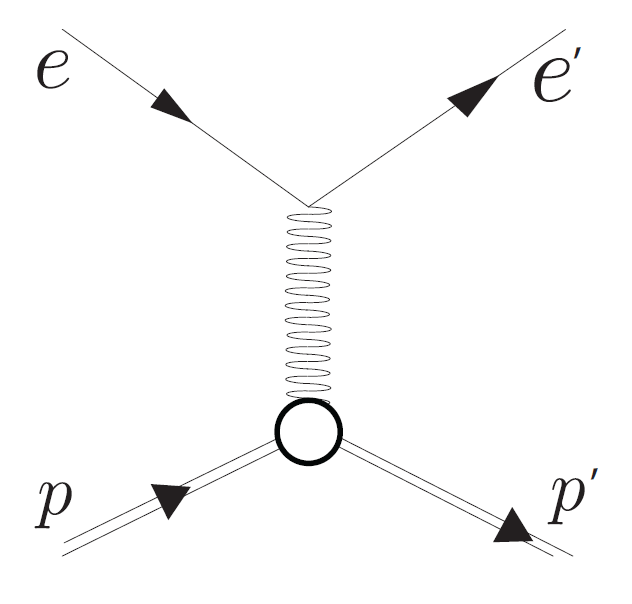
\includegraphics[width=0.5\textwidth]{Chapters/Ch1-Intro/Ch1-Sec1-Background/pics/elastic_feynamn.png}
            \caption{Tree-level elastic scattering Feynman diagram}
        \end{figure}

        The momentum transfer \textit{q} sets the resolution scale for these processes, but it is convenient to work with the negative square of this value, defined as $Q^2 = -q^2$. With this term, we can express the relativistic differential cross section for the scattering of electrons off a resting, point-like proton as in Eq. \ref{eq:FullElastic}, where $m_p$ is the mass of the proton. 

            \begin{equation}\label{eq:FullElastic}
                    \frac{d\sigma}{d\Omega} = \frac{\alpha^2}{4E_{beam}^2\sin^4{(\theta/2)}} \frac{E_{e'}}{E_{beam}} ( \cos^2{\frac{\theta}{2}} + \frac{Q^2}{2m_p^2}\sin{\frac{\theta}{2}}^2 )
            \end{equation}
            \myequations{Elastic Scattering Differential Cross Section}


            Compared with Mott Scattering, there are two differences in this formula: The $\frac{E_{e'}}{E_{beam}}$ term in the scattering cross section comes from the electron losing energy to the proton's final state kinetic energy (no longer fixed), and the term proportional to $\sin^2(\theta/2)$ is due to a purely magnetic spin-spin interaction. 


            \indent If the proton were a point, then Eq. \ref{eq:FullElastic} would agree with experiment for all electron scattering energies. Instead, deviations are observed as we increase the beam energy. To account for this structure, we need to include two form factors, $G_E(Q^2)$ - related to the distribution of charge, and $G_M(Q^2)$, related to the distribution of the magnetic moment inside the proton. In the low-$Q^2$ limit, these form factors are the Fourier transforms of the charge an magnetic moment distributions as in Eq. \ref{eq:GE} and \ref{eq:GM}, reducing to the charge and the magnetic moment of the proton in the $Q^2$ = 0 limit. %but the carryover is not exact in general due to being functions of the 4-momenta, instead of 3 momenta. E.g.:

        \begin{equation}\label{eq:GE}
             G_E(Q^2) \approx G_E(q^2) = \int e^{iq\cdot r} \rho (r) d^3r  \quad \quad   G_E(0) = \int  \rho (r) d^3r = 1
        \end{equation}

        \begin{equation}\label{eq:GM}
             G_M(Q^2) \approx G_E(q^2) = \int e^{iq\cdot r} \mu (r) d^3r  \quad \quad   G_M(0) = \int  \mu (r) d^3r = 2.79
        \end{equation}
        
        
        Including these form factors in our cross section gives us the full elastic scattering cross section, as shown in Eq. \ref{eq:rosenbluth}.
                
        \begin{equation}\label{eq:rosenbluth}
            \frac{d\sigma}{d\Omega} = \frac{\alpha^2}{4E_1^2\sin^4{(\theta/2)}}\frac{E_3}{E_1}\left( \frac{G_E^2+\tau G_M^2}{1+\tau} \cos^2{\frac{\theta}{2}}+2\tau G_M^2\frac{Q^2}{2m_p^2}\sin^2(\frac{\theta}{2})\right)
        \end{equation}
       \myequations{Rosenbluth Scattering Cross Section}
       
        Where $\tau = \frac{Q^2}{4m_p^2}$.
        

        \begin{figure}[H]\label{fig:formfactors}
            \centering
            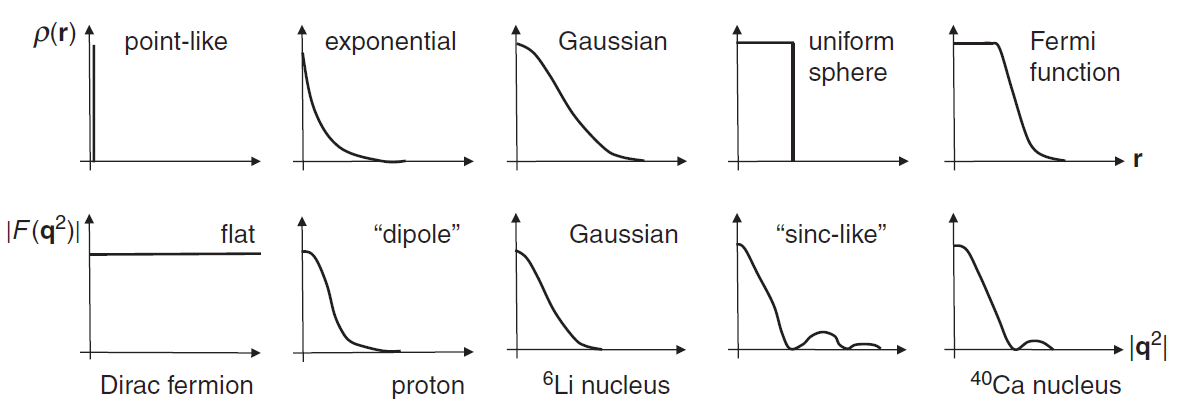
\includegraphics[width=0.9\textwidth]{Chapters/Ch1-Intro/Ch1-Sec1-Background/pics/intro/possibleformfactors.png}
            \caption[Fourier Transforms of Charge Distributions]{Samples of charge distributions and their corresponding form factors $F(\textbf{q}^2)$, from \cite{Thomson2013ModernPhysics} }
        \end{figure}
        

                By the 1960s, elastic scattering had been studied sufficiently well as to measure the proton form factors up to several GeV in $Q^2$. The observed results were consistent with a proton having a `dipole' form factor, as shown in Fig. \ref{fig:formfactors}. Investigating proton structure at finer spatial resolutions requires increasing the beam energy, but eventually the the elastic scattering cross section becomes negligible and instead the interactions are sufficiently energetic so as to create additional particles.
                
            %Also something about this is only valid due to angular momentum preservation for 1 photon exchange. 


    \subsection{Inelastic Scattering and Parton Distribution Functions}

        Elastic scattering can be defined as interactions where the target stays intact; specifically, the variable $W=p_p+q$ is the four-momentum of the outgoing struck target, where elastic scattering satisfies the condition $W^2 =m_p^2$. If $W^2$ \> $m_p^2$, we instead have inelastic scattering, written as ep$\rightarrow$eX, where X stands for some outgoing hadronic system, as shown in the Feynman diagram in Fig. \ref{fig:FeynmanInelastic}.    



    
        \begin{figure}\label{fig:FeynmanInelastic}
            \centering
            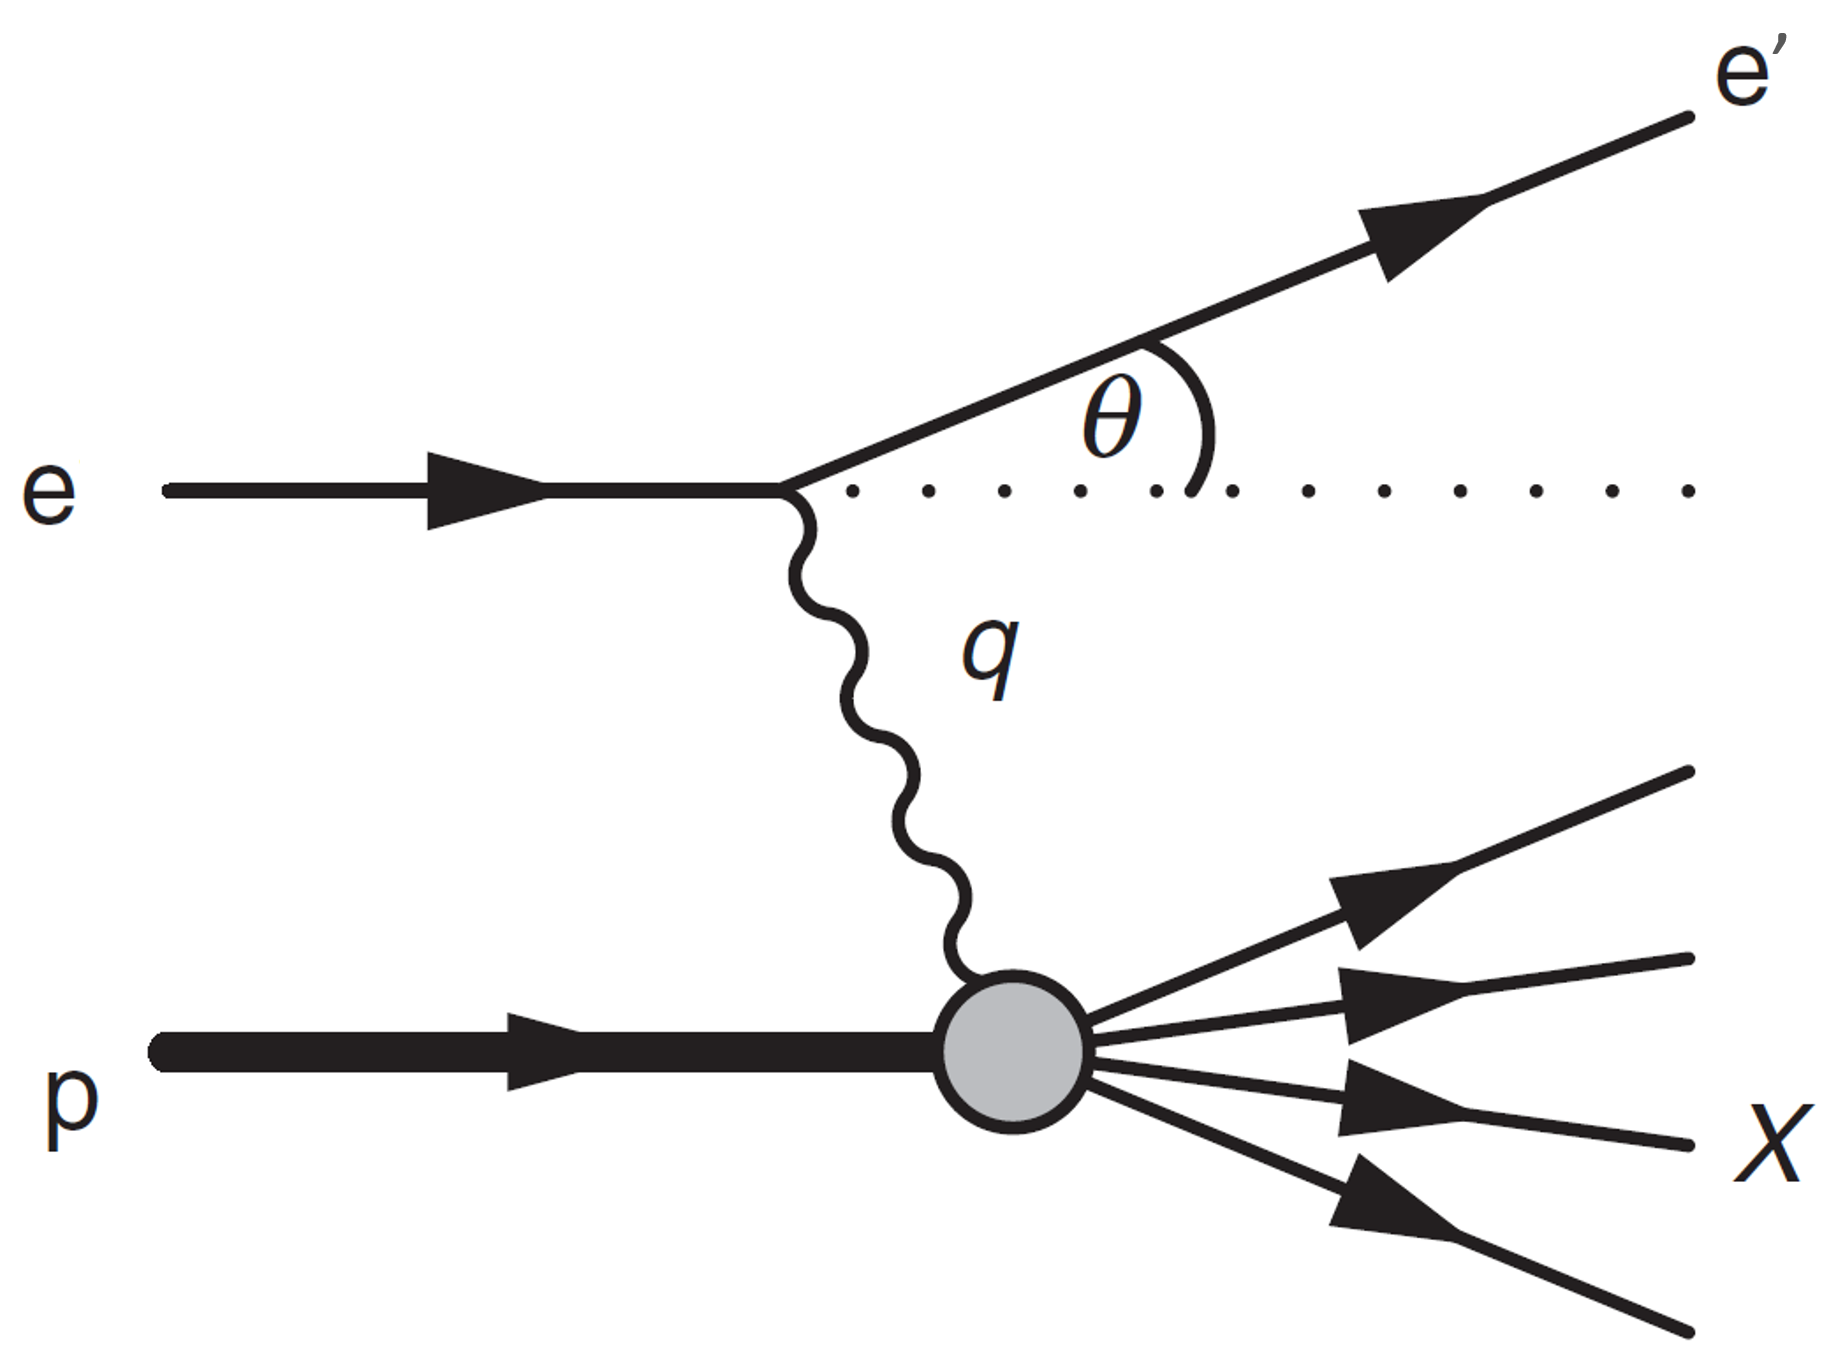
\includegraphics[width=0.5\textwidth]{Chapters/Ch1-Intro/Ch1-Sec1-Background/pics/inelastic-ep/eppx.png}
            \caption[Diagram]{Diagram}
        \end{figure}

        In general, 

        \begin{figure}
            \centering
            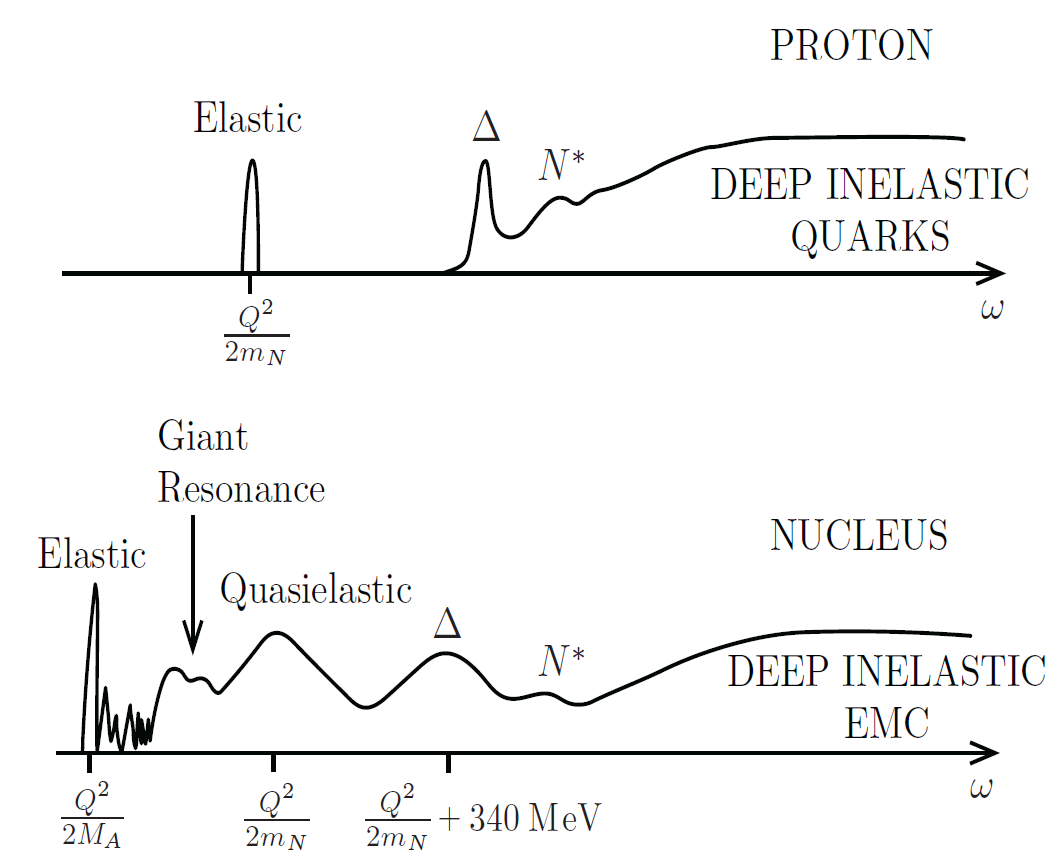
\includegraphics[width=0.5\textwidth]{Chapters/Ch1-Intro/Ch1-Sec1-Background/pics/intro/scatcrosstheory.png}
            \caption[Scattering Cross Section vs. Energy Transfer]{Sketch of cross section as a function of electron energy transfer for inclusive electron scattering off a proton (top) and a nucleus (bottom), from \cite{Donnelly2017FoundationsPhysics} }
            \label{fig:ScatteringvsW}
        \end{figure}


        Since we remove the constraint that the mass of the final state is the proton mass, we now have one extra degree of freedom, i.e., we need 2 variables to describe inelastic scattering. These are usually Bjorken X $x_B$ and the 4-momentum transfer of the virtual photon $Q^2$.\\
        $x_B$ is a measure of elasticity - 1 for elastic scattering. Also, is the fraction of proton momentum carried by the struck quark in the infinite momentum frame.       Think of Xb as the ratio of momentum transfer to energy transfer. 
        
        \begin{equation}
            x = \frac{Q^2}{2p_2\cdot q} = \frac{Q^2}{Q^2+W^2-m_p^2}
        \end{equation}\myequations{Bjorken X}

        The Deep Inelastic Scattering regime is defined by kinematics as $Q^2$ \> 1 GeV$^2$ and W$^2$\>4 GeV$^2$
        
    

    
            Derivation of infinite momentum frame Bjorken x. Take quark to have momentum fraction $\xi$ of proton's total momentum,i.e. $p_q = \xi p_2$:\\
            \indent Inf. Mom. frame - neglect proton mass so $p_2$ = $E_2$, neglect all transverse momenta:\\
            \indent Struck quark 4-momenta: $p_q = \xi p_2 = (\xi E_2, \xi E_2, 0, 0)$\\
            \indent 4-momenta of quark after interaction: $(p_q + q) = (\xi p_2 +q)$\\
            \indent Square the 4-momenta $(\xi p_2 +q)^2 = \xi^2 p_2^2 +q^2 + 2\xi p_2 \cdot q  = m_q^2$\\
            \indent Continue, noting $p_q = \xi p_2$ : $m_q^2 = p_q^2 - Q^2 + 2 \xi p_2 \cdot q$\\
            \indent Since $p_q^2$ = $m_q^2$, we have: $m_q^2 = m_q^2 -Q^2 + 2 \xi p_2 \cdot q$\\
            \indent So $0 = -Q^2 + 2\xi p_2 \cdot q \longrightarrow \xi = \frac{Q^2}{2 p_2 \cdot q} = x_B$\\
        
        
        y is a measure of the inelasticity of the scattering, it is the fractional energy lost by the electron in the scattering process (second equality is true where proton is at rest). 0 is for perfectly elastic, 1 is for entirely inelastic. 
        
        \begin{equation}
            y = \frac{p_2 \cdot q}{p_2 \cdot p_1} = 1 - \frac{E_3}{E_1}
        \end{equation}
        

We get quark PDFs from the F2 structure function. How do we get gluon PDFs? Can we probe the gluon directly? Does it coulple to the photon? No! We assume QCD evolution equations (e.g. DGLAP) and gluon dist comes out. 


            W is the four momenta of the final state system that started with the proton, W = q + $p_2$. It is useful as $W^2 = m_p^2 -Q^2 + 2 p_2 \cdot q$
        
        \indent To describe further proton sub-structure, we need to introduce structure functions, $F_1(x,Q^2)$ - purely magnetic, and $F_2(x,Q^2)$. For DIS where $Q^2 >> m_p^2y^2$, we have the following cross section formula:
        
        \begin{figure}[H]
            \centering
            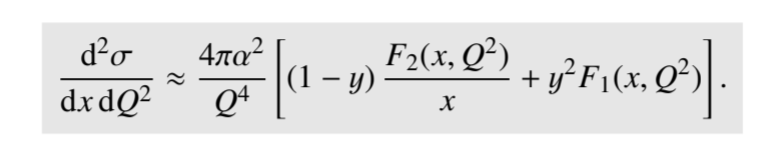
\includegraphics[width=10cm]{Chapters/Ch1-Intro/Ch1-Sec1-Background/pics/inelastic-ep/dis-xsection.PNG}
            \caption{General DIS cross section}
        \end{figure}

        \indent In DIS, we observe Bjorken scaling and Callan-Gross
        
        \begin{figure}[H]
            \centering
            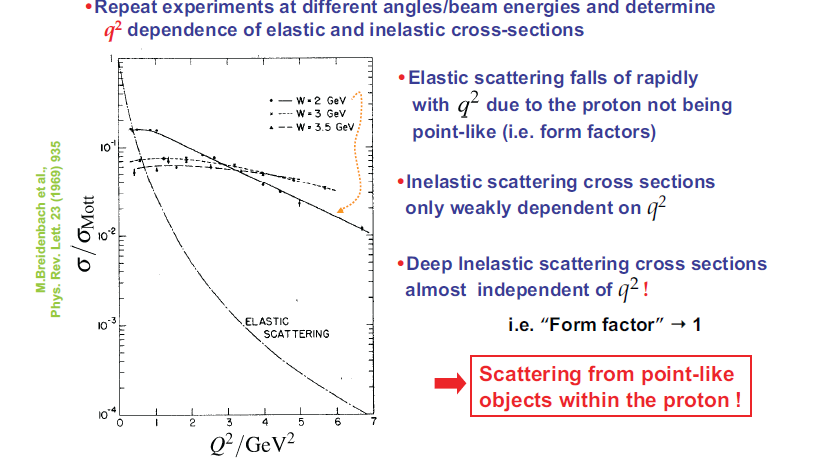
\includegraphics[width=10cm]{Chapters/Ch1-Intro/Ch1-Sec1-Background/pics/inelastic-ep/DIS.png}
            \caption{Early Bjorken Scaling Example}
        \end{figure}
        
        After performing DIS measurements at SLAC with electron energies between 5 and 20 GeV on liquid hydrogen, using a movable spectrometer over various angles, showed two important results:\\
        \newline
        \textbf{Bjorken Scaling} where $F_1$ and $F_2$ are basically flat with respect to $Q^2$, and thus are independent of $Q^2$, indicating that we are scattering off point-like constituents inside the proton.\\
        \newline
        \textbf{Callan Gross Relation} where $F_2 = 2x F_1$, a relation which can be explained by assuming the underlying process is actually elastic scattering off of point-like spin-half constituents inside the prton (quarks). 

        \indent These describe the distribution of quarks within the nucleon. Describes the momentum fraction distribution of quarks. For example:\\
        \newline
        $u^p(x)dx$\\
        \newline
        Represents the number of up-quarks within the proton with momentum fraction between x and dx. The functional forms of the PDFs are not a-priori known. Some potential PDFs could be as shown below:\\
        
        \begin{figure}[H]
            \centering
            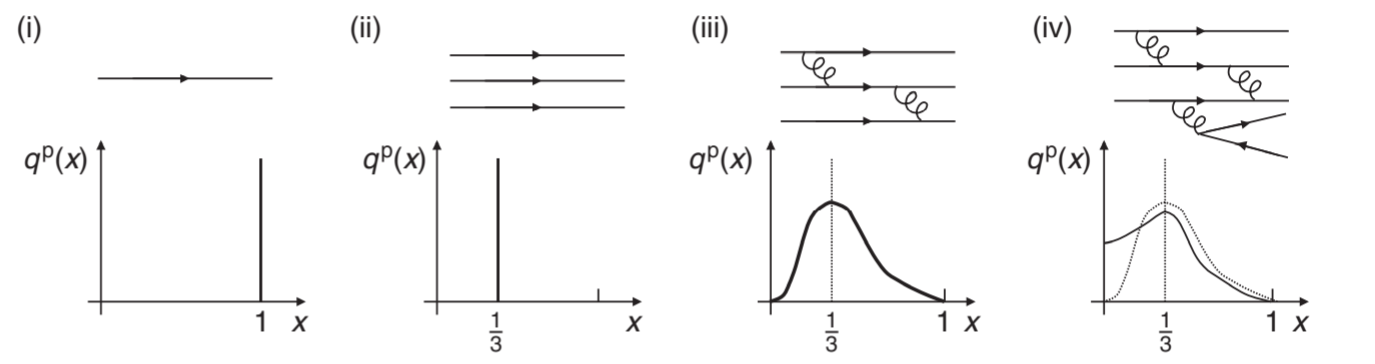
\includegraphics[width=12cm]{Chapters/Ch1-Intro/Ch1-Sec1-Background/pics/inelastic-ep/pdf-possibilities.PNG}
            \caption{Potentail PDFs}
        \end{figure}
        
        (i) - if the proton consisted of a single quark\\
        (ii) - if the proton had 3 static quarks\\
        (iii) - quarks interacting and Heisenberg uncertainty (momentum smearing)\\
        (iv) - interacting quarks with higher order diagrams - gluons produced, so enhances low x part of PDF\\
        \newline
        We can access these distributions experimentally as the parton model predicts the the cross section for elastic scattering off of quarks with charge $Q_i$ and momentum fraction in the range of x to x + dx as:
        
               
        \begin{figure}[H]
            \centering
            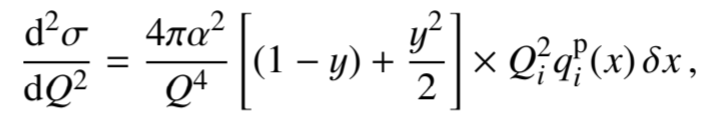
\includegraphics[width=8cm]{Chapters/Ch1-Intro/Ch1-Sec1-Background/pics/inelastic-ep/quark-x.PNG}
            \caption{Quark scattering cross section}
        \end{figure}
        
        So then the cross section summing over all quark flavours is:
        
               
        \begin{figure}[H]
            \centering
            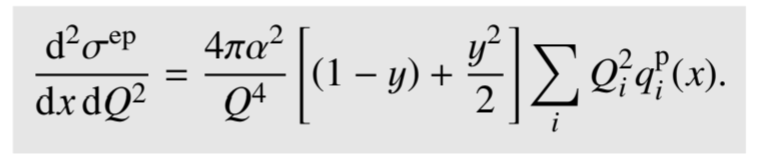
\includegraphics[width=8cm]{Chapters/Ch1-Intro/Ch1-Sec1-Background/pics/inelastic-ep/quark-x-sum.PNG}
            \caption{Quark PDF - cross section relation}
        \end{figure}
        
        and comparing it with the general expression for DIS cross section:
        
                
        \begin{figure}[H]
            \centering
            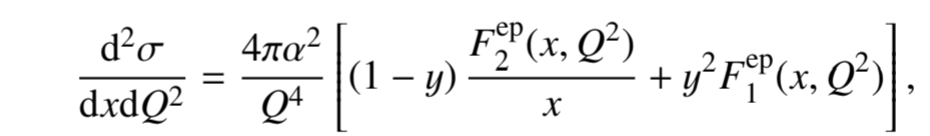
\includegraphics[width=8cm]{Chapters/Ch1-Intro/Ch1-Sec1-Background/pics/inelastic-ep/inel-general.PNG}
            \caption{General DIS cross section}
        \end{figure}
        We see we can get the relation:
        
                
        \begin{figure}[H]
            \centering
            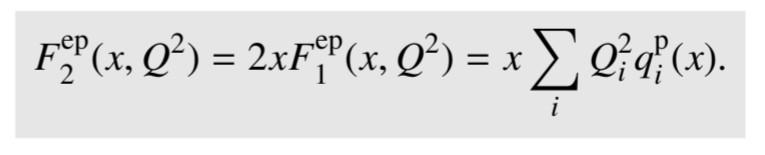
\includegraphics[width=8cm]{Chapters/Ch1-Intro/Ch1-Sec1-Background/pics/inelastic-ep/f2-sum-q.PNG}
            \caption{Structure function - quark PDF relatio}
        \end{figure}
        
        For an explicit example, we have (neglecting heavier quarks, which have smaller contributions):
        
                
        \begin{figure}[H]
            \centering
            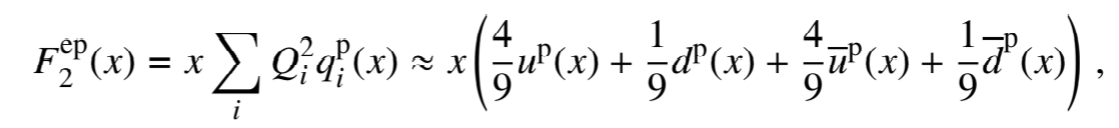
\includegraphics[width=12cm]{Chapters/Ch1-Intro/Ch1-Sec1-Background/pics/inelastic-ep/example-f2.PNG}
            \caption{Up and Down quark contributions to structure functions}
        \end{figure}
        
        Note that the parton model predicts both Bjorken scaling and the Callan Gross relation. Importantly, because QCD is hard, the PDFs cannot be calculated from perterbation theroy, and must be measured in DIS. We can integrate the PDFs to determine the total momentum fraction of the proton carried by each flavour of quark, as:
        
                
        \begin{figure}[H]
            \centering
            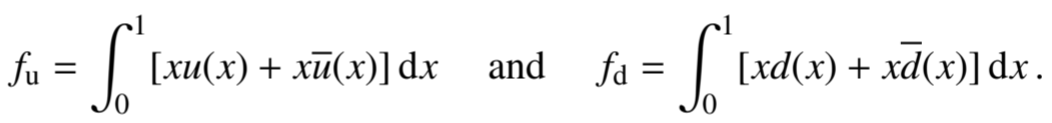
\includegraphics[width=12cm]{Chapters/Ch1-Intro/Ch1-Sec1-Background/pics/inelastic-ep/integrated-ud.PNG}
            \caption{Total quark momentum fractions}
        \end{figure}
        
        Doing this after DIS measurements yields $f_u = 0.36$ and $f_d = 0.18$, so the u and d quarks only carry about half of the total momentum of the proton. The rest is carried by gluons, which do not interact in QED ep scattering. \\
        
    
        
        Structure functions were studied in great detail (one million DIS events at $Q^2$ greater than 200 GeV$^2$ - kinematic range was up to $Q^2 = 20,000 GeV^2$ and $x < 0.0001$. $Q^2$ and $x$ were determined solely by precisely measuring the scattering angle and energy of the electron. 
        
        \begin{figure}[H]
            \centering
            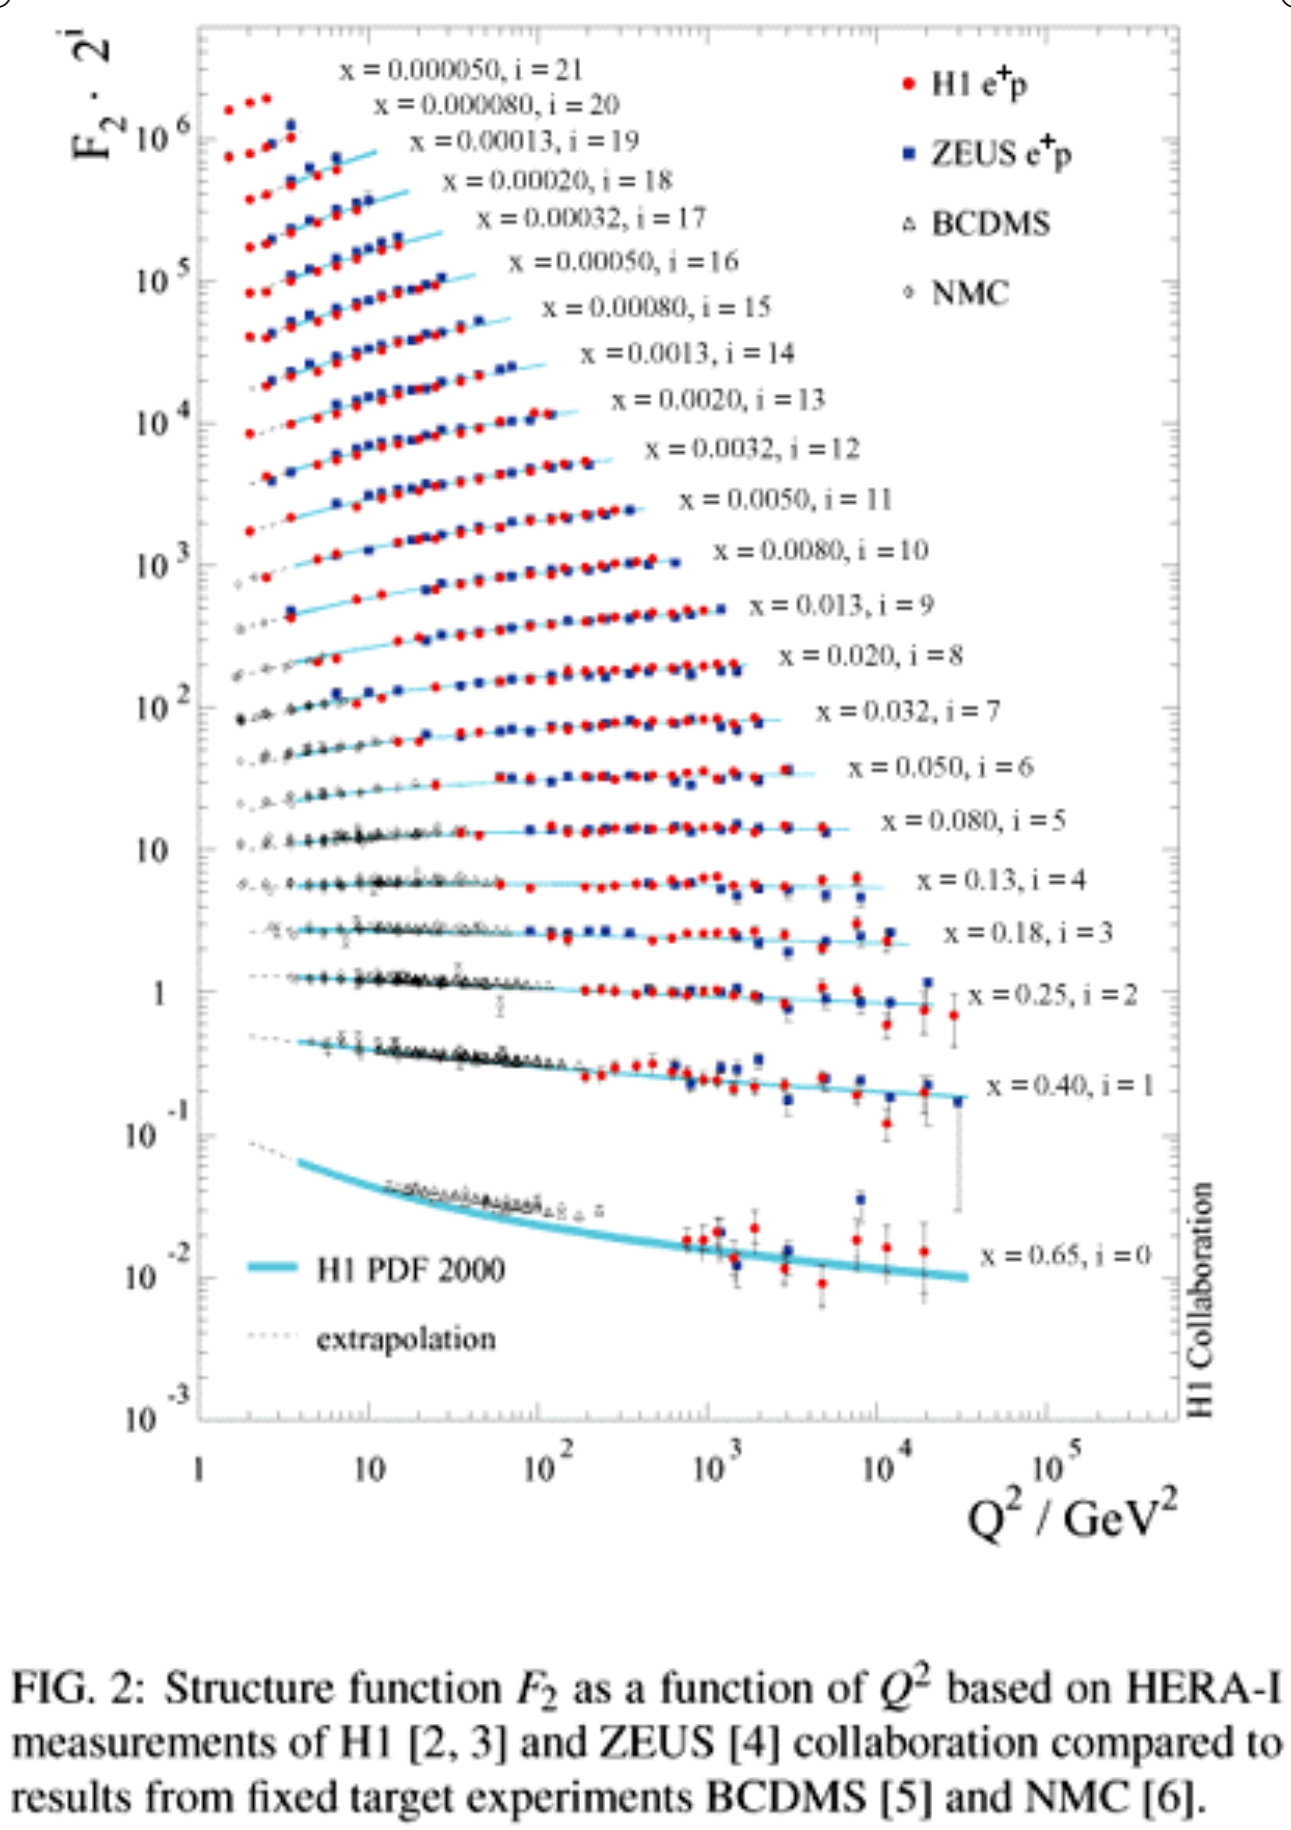
\includegraphics[width=10cm]{Chapters/Ch1-Intro/Ch1-Sec1-Background/pics/inelastic-ep/Hera-dis.PNG}
            \caption{HERA structure functions}
        \end{figure}
        
        2 important takeaways:\\
        \newline
        1- Bjorken scaling holds up to $Q^2 = 20,000$ GeV$^2$, implying that quarks are point like up to scales of at least $10^{-18}$m. \\
        \newline
        2- \textbf{Scaling violations: }\\
        \newline
        \indent At medium X, we are independent of Q2, indicating we have quarks. At high x, the $F_2$ structure function decreases at high x, and increases at low x, with increasing $Q^2$. More specifically, imagine measuring the $F_2$ structure function across x at a certain $Q^2$. Now measure again at a higher $Q^2$. You will see the curve is shifted higher at low x, and lower at high x:
        
                
        \begin{figure}[H]
            \centering
            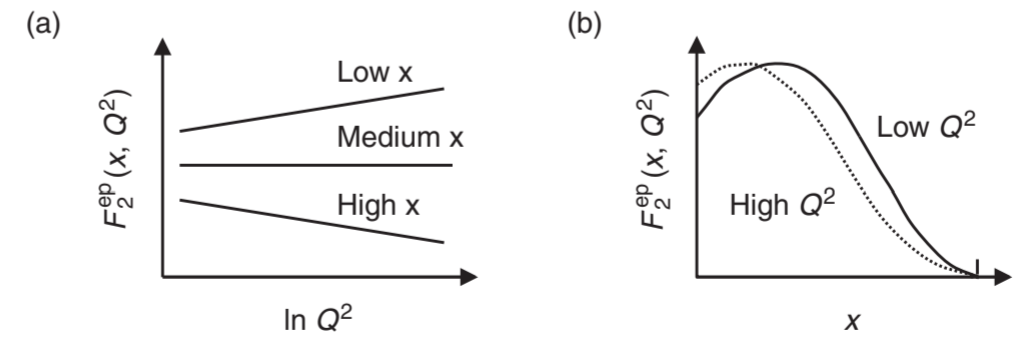
\includegraphics[width=12cm]{Chapters/Ch1-Intro/Ch1-Sec1-Background/pics/inelastic-ep/scaling-violations.PNG}
            \caption{Explaination of Scaling Violations}
        \end{figure}
        
        This is indicative of the fact that at higher $Q^2$, the proton has a greater fraction of low x quarks. I.e., at low $Q^2$ we do not "see" the low-x quarks, but as we increase our resolving power, we do.\\
        \newline
        N.b. - we cannot measure the gluon PDFs, but can model them with QCD parton evolution equations such as DGLAP or BFKL.\\
        \newline
        Finally, we include a proton PDF at $Q^2$ = 10 GeV$^2$ and at $10^4$ GeV$^2$. (note - on a semilog plot!)
        
               
        \begin{figure}[H]
            \centering
            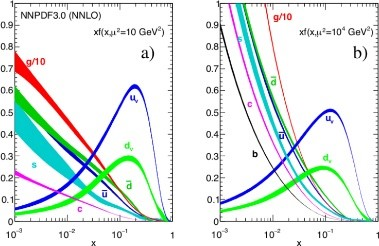
\includegraphics[width=14cm]{Chapters/Ch1-Intro/Ch1-Sec1-Background/pics/inelastic-ep/PDFs.jpg}
            \caption{PDFs at two different $Q^2$ values}
        \end{figure}

     PDFs allow for a 1 dimensional picture of the inner workings of a proton - proton femtography. Even more informaiton can be gleaned from scattering reactions. In particular, efforts are now directed towards so called nuclear tomography - 3D imaging of nucleon structure.  

\clearpage
